% !TeX program = lualatex
% ================================================================
% Polish Tier 3 Vocabulary Version of RatioChallengeSheet
%
% Generated by the server using the following settings:
%
%   language            Polish (pol)
%   text direction      left to right
%   font                Noto Serif
%   fallback font       Noto Serif
%   built from          latex/worksheets/ratioAndProportion/ratioChallengeSheet.tex
%   vocabulary key      latex/worksheets/ratioAndProportion/ratioChallengeSheet/L2/pol/ratioChallengeSheet_polishKey.tex
%   tier 3 vocabulary   green   RGB 0 128 0
%   English text        black   RGB 0 0 0
%   Polish text         purple  RGB 112 48 160
%   layout macros       version 3
%
% Please don't edit any information in this comment block - the server
% compares it against the current settings and rebuilds this file when
% they differ, so changes here would be overwritten. However, feel free
% to make updates to the LaTeX below if you want to edit it.
% ================================================================

\documentclass[11pt,a4paper]{article}
% ================================================================
% Copied from the English sheet this was translated from, so that
% anything it sets up for itself still works here
% ================================================================
\usepackage[a4paper,top=11mm,bottom=10mm,left=14mm,right=14mm]{geometry}
\usepackage[T1]{fontenc}
\usepackage{amsmath}
\usepackage{amssymb}
\usepackage{enumitem}
\usepackage{multicol}
\usepackage{array}
\usepackage{tikz}
\usepackage[most]{tcolorbox}
\usetikzlibrary{arrows.meta,matrix}

% ================================================================
% Challenge: ratio and the shape of A4 paper.
%
% A four-page challenge sheet on ratio for confident pupils who know
% Pythagoras' theorem and surds. The quadratic equations are solved by
% rearranging a completed-square form that the sheet gives as a fact, so
% the quadratic formula is not needed. It is built on
% one idea: when a shape is cut into pieces that are similar to the
% whole shape, the rule for cutting it fixes the ratio of its lengths.
% Similar rectangles have equivalent ratios short : long, so the method
% throughout is to write both ratios in the form 1 : n and set them
% equal. Equivalent ratios and equations are both worked with curved
% arrows that show the same operation done to both sides.
%
% The first pages are discovery. The key idea box shows folding, similar
% shapes and equivalent ratios in pictures. Q1 writes scale drawings of
% A3, A4 and A5 in the form 1 : n. Q2 folds other rectangles in half,
% and finds the two that the shape that stays the same lies between. Q3
% practises equivalent ratios, and shows that the second part divided
% by the first part is the same for equivalent ratios. Q4 is open:
% pupils set up and solve the equation for 1 : sqrt(2) themselves, with
% only the hint that the whole and half sheets have equivalent ratios.
%
% Part 1 (Q5 to Q8) uses the ratio with real paper: US Letter, the sizes
% A0 to A6, photocopier percentages, and a fold that shows the ratio on
% a real sheet.
%
% Part 2 changes the rule: three strips (Q9, the method of Q4 again, with
% the picture and lines for the two ratios but no other scaffold), then
% n strips, the golden rectangle (one square cut off) and the silver
% rectangle (a square cut off A4).
% Q13 moves to triangles and an L-shape, and asks why n similar pieces
% always give 1 : sqrt(n).
%
% Page 4 goes into more dimensions: a box that halves into two similar
% boxes is 1 : cbrt(2) : cbrt(4) (Q14), and the four-dimensional box is
% 1 : 2^(1/4) : 2^(1/2) : 2^(3/4) (Q15). Q16 collects the pattern and
% asks what happens as the number of dimensions grows. Q17 is the
% A-series spiral and the sum 1/2 + 1/4 + 1/8 + ... = 1. Q18 is the
% family x^2 - kx - 1 = 0, solved from its completed-square form, and an
% open task.
%
% There is little working space, so pupils work on paper. The answers
% are in a comment beside each question.
% ================================================================

\pagestyle{empty}
\linespread{1.04}\selectfont
\setlength{\parskip}{3pt}
\setlength{\parindent}{0pt}
\renewcommand{\arraystretch}{1.25}
\setlist[enumerate,1]{label=\textbf{Q\arabic*.}, leftmargin=*, itemsep=6pt,
  topsep=2pt, partopsep=0pt, parsep=2pt}
\setlist[enumerate,2]{label=(\alph*), leftmargin=*, itemsep=2pt, topsep=2pt,
  partopsep=0pt, parsep=1pt}
\setlength{\multicolsep}{2pt}

% Gaps to write in: \gap inside a sentence, \tgap inside a table,
% \eqgap inside a ratio or an equation, and \opgap for an operation
% beside a curved arrow. \gapstrut makes a table row tall enough to
% write in.
\newcommand{\ansline}[1][2.2cm]{\underline{\hspace{#1}}}
\newcommand{\gap}{\ansline[1.1cm]}
\newcommand{\tgap}{\ansline[0.8cm]}
\newcommand{\eqgap}{\underline{\hspace{1.0cm}}}
\newcommand{\opgap}{\underline{\hspace{0.55cm}}}
\newcommand{\gapstrut}{\rule[-2mm]{0pt}{7mm}}

% The idea the sheet is built on, in a box that is tinted only faintly
% so that the printed sheet uses little toner.
\newtcolorbox{keyidea}{colback=orange!3,colframe=orange!35,boxrule=0.6pt,
  left=6pt,right=6pt,top=2pt,bottom=2pt}

% The part headings: a thick rule, the title and a thin rule.
\newcommand{\parttitle}[2]{%
  \par\vspace{4pt}%
  {\color{blue!45!black}\hrule height 1pt}\vspace{3pt}%
  {\large\bfseries Part #1: #2\par}\vspace{2pt}%
  {\color{blue!45!black}\hrule height 0.4pt}\vspace{3pt}}

% A small bold title above a working.
\newcommand{\worktitle}[1]{{\small\bfseries #1}\par\vspace{1pt}}

% Doing the same thing to both sides, for an equation or for the parts
% of a ratio. The lines are the rows of a matrix, lined up on the equals
% sign or the colon, and a curved arrow on each side goes from one line
% to the next, with the operation beside it. The operations are a list,
% one for each step:
%   \bothsides{x \& = \& \dfrac{2}{x}\\ x^2 \& = \& 2\\}{\times x}
%   \bothsides{0.75 \& : \& 1\\ 1 \& : \& 1.333\\}{\div0.75}
% A ratio with three parts uses the option ratio3:
%   \bothsides[ratio3]{a \& : \& b \& : \& c\\ ...}{...}
% An operation given as \opgap is left for pupils to write in.
\tikzset{
  bsline/.style  = {matrix of math nodes, ampersand replacement=\&,
                    row sep=0.55em, column sep=0.2em,
                    nodes={inner sep=1pt},
                    column 1/.style={anchor=base east},
                    column 2/.style={anchor=base},
                    column 3/.style={anchor=base west}},
  ratio3/.style  = {column 3/.style={anchor=base},
                    column 4/.style={anchor=base},
                    column 5/.style={anchor=base west}},
  bsarrow/.style = {-{Stealth[length=4pt]}, blue!55!black, semithick},
  bslab/.style   = {font=\small, text=blue!55!black, inner sep=1.5pt},
}
\newcommand{\bothsides}[3][]{%
  \begin{tikzpicture}[baseline=(m-1-2.base)]
    \matrix (m) [bsline, #1] {#2};
    \foreach \op [count=\i, evaluate=\i as \j using int(\i+1)] in {#3} {
      \draw[bsarrow] ([xshift=-3pt]m.west |- m-\i-2.center) to[bend right=50]
        node[bslab, left] {$\op$} ([xshift=-3pt]m.west |- m-\j-2.center);
      \draw[bsarrow] ([xshift=3pt]m.east |- m-\i-2.center) to[bend left=50]
        node[bslab, right] {$\op$} ([xshift=3pt]m.east |- m-\j-2.center);
    }
  \end{tikzpicture}}

% A rectangle with short side 1 and long side n, cut into k equal strips
% across its long side, with one strip drawn beside it.
%   \cutdiagram{k}{n}{label of the long side}{label of a strip's short side}{word}
\newcolumntype{C}[1]{>{\centering\arraybackslash}p{#1}}
\newcommand{\cutdiagram}[5]{%
  \begin{tikzpicture}[baseline=(current bounding box.north), font=\small]
    \pgfmathsetmacro{\sw}{1.0}
    \pgfmathsetmacro{\lh}{1.0*#2}
    \pgfmathsetmacro{\st}{\lh/#1}
    \draw[thick, fill=blue!3] (0,0) rectangle (\sw,\lh);
    \foreach \k in {1,...,#1} {\ifnum\k<#1
      \draw[dashed] (0,\k*\st) -- (\sw,\k*\st);\fi}
    \node[below] at (\sw/2,0) {$1$};
    \node[left] at (0,\lh/2) {#3};
    \draw[-{Stealth[length=4pt]}, gray] (\sw+0.1,\lh/2) --
      node[above, font=\scriptsize, text=black] {#5} (\sw+0.7,\lh/2);
    \draw[thick, fill=blue!3] (\sw+1.55,\lh/2-\st/2) rectangle
      (2*\sw+1.55,\lh/2+\st/2);
    \node[below] at (1.5*\sw+1.55,\lh/2-\st/2) {$1$};
    \node[left] at (\sw+1.55,\lh/2) {#4};
  \end{tikzpicture}}

% A scale drawing of a sheet of paper at 1 : 20, with its name inside and
% its sides labelled in millimetres. Every drawing has the same height,
% so that drawings of different sizes stand on the same line.
%   \papersheet{short side in mm}{long side in mm}{name}
\newcommand{\papersheet}[3]{%
  \begin{tikzpicture}[font=\small]
    \path (0,-0.4) -- (0,2.15);
    \draw[thick, fill=blue!3] (0,0) rectangle (#1/200,#2/200);
    \node[font=\scriptsize] at (#1/400,#2/400) {#3};
    \node[below, font=\scriptsize] at (#1/400,0) {$#1$\,mm};
    \node[left, font=\scriptsize] at (0,#2/400) {$#2$\,mm};
  \end{tikzpicture}}

% One of the rectangles in Q2: the whole sheet, the working that writes
% the half sheet in the form 1 : n, and whether the shape is the same.
%   \foldcell{whole sheet ratio}{working}{answer or gap}
\newcommand{\foldcell}[3]{%
  \begin{minipage}[t]{0.48\linewidth}
  \centering
  \worktitle{Whole sheet $#1$. Half sheet, short : long:}
  #2\hspace{0.8em}{\small Same shape?\ \ #3}
  \end{minipage}}

% Characters this language's font has not got are borrowed from another,
% rather than being silently dropped - see docs/translated-sheet-latex.md
\directlua{%
  if luaotfload and luaotfload.add_fallback then
    luaotfload.add_fallback("eallatinfallback",
      { "Noto Serif:mode=harf;" })
  else
    tex.error("this luaotfload is too old to register a fallback font")
  end
}
\usepackage[english]{babel}
\babelprovide[import]{polish}
\babelfont[polish]{rm}[Renderer=Harfbuzz, BoldFont={Noto Serif}, ItalicFont={Noto Serif}, BoldItalicFont={Noto Serif}, RawFeature={fallback=eallatinfallback}]{Noto Serif}
\babelfont[polish]{sf}[Renderer=Harfbuzz, BoldFont={Noto Serif}, ItalicFont={Noto Serif}, BoldItalicFont={Noto Serif}, RawFeature={fallback=eallatinfallback}]{Noto Serif}
\newcommand{\ealtext}[1]{\foreignlanguage{polish}{#1}}
\newcommand{\ealtextblock}[1]{{\raggedright\foreignlanguage{polish}{#1}\par}}
% ================================================================
% EAL layout helpers
% ================================================================
\usepackage{xcolor}

\definecolor{ealkeycolour}{RGB}{0,128,0}
\definecolor{ealenglish}{RGB}{0,0,0}
\definecolor{ealtwocolour}{RGB}{112,48,160}

\newsavebox{\ealboxen}
\newsavebox{\ealboxtr}
\newlength{\ealglosswd}
\newlength{\ealglossraise}
\setlength{\ealglossraise}{1.15em}

% a tier 3 word, in English and in translation alike
\newcommand{\ealkey}[1]{\textcolor{ealkeycolour}{#1}}
\newcommand{\ealkeytr}[1]{\textcolor{ealkeycolour}{\ealtext{#1}}}

% One translated word above one English word. Built from kernel
% primitives, never a tabular, which would break wherever the sheet
% loads array, booktabs or tabularx. The box is as wide as the wider of
% the two, so a long translation pushes its neighbours aside instead of
% overlapping them, and it claims its full height so a table row or a
% TikZ node makes room for it.
\newcommand{\ealgloss}[2]{%
  \sbox{\ealboxen}{\ealkey{#1}}%
  \sbox{\ealboxtr}{\small\textcolor{ealtwocolour}{\ealtext{#2}}}%
  \setlength{\ealglosswd}{\wd\ealboxen}%
  \ifdim\wd\ealboxtr>\ealglosswd\setlength{\ealglosswd}{\wd\ealboxtr}\fi
  \leavevmode
  \makebox[\ealglosswd][c]{%
    \makebox[0pt][c]{\usebox{\ealboxen}}%
    \makebox[0pt][c]{\raisebox{\ealglossraise}{\usebox{\ealboxtr}}}%
  }%
}

% opens up line spacing around a block of glosses, so the raised
% translations sit clear of the line above
\newenvironment{ealglossed}{\par\linespread{2.1}\selectfont\ignorespaces}{\par}

% a whole translated sentence above its English counterpart. block level,
% so it does not belong inside a tabular cell
\newcommand{\ealpara}[2]{%
  \par\addvspace{0.5\baselineskip}%
  {\color{ealtwocolour}\ealtextblock{#1}}%
  \penalty200
  {\color{ealenglish}#2\par}%
  \addvspace{0.5\baselineskip}%
}

\begin{document}

\begin{ealglossed}
\begin{center}
  {\Large\bfseries Challenge: \ealgloss{Ratio}{Stosunek} and the Shape of A4 Paper}
\end{center}
\end{ealglossed}
\vspace{-6pt}

\begin{keyidea}
\small
\begin{minipage}[t]{0.35\linewidth}
\centering
\textbf{Folding}\par\vspace{4pt}
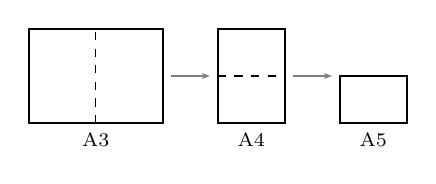
\begin{tikzpicture}[font=\scriptsize]
  \draw[thick, fill=white] (0,0) rectangle (1.7,1.2);
  \draw[dashed] (0.85,0) -- (0.85,1.2);
  \node[below] at (0.85,0) {A3};
  \draw[-{Stealth[length=3pt]}, gray] (1.8,0.6) -- (2.3,0.6);
  \draw[thick, fill=white] (2.4,0) rectangle (3.25,1.2);
  \draw[dashed] (2.4,0.6) -- (3.25,0.6);
  \node[below] at (2.825,0) {A4};
  \draw[-{Stealth[length=3pt]}, gray] (3.35,0.6) -- (3.85,0.6);
  \draw[thick, fill=white] (3.95,0) rectangle (4.8,0.6);
  \node[below] at (4.375,0) {A5};
\end{tikzpicture}\par\vspace{2pt}
{\footnotesize Folding a sheet in half halves its long side, and makes the
next size.}
\end{minipage}\hfill
\begin{minipage}[t]{0.29\linewidth}
\begin{ealglossed}
\centering
\textbf{\ealgloss{Similar}{Podobne} shapes}\par\vspace{4pt}
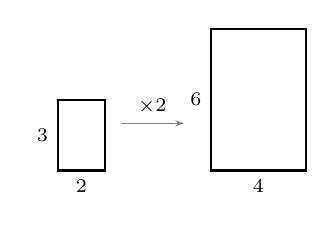
\begin{tikzpicture}[font=\scriptsize]
  \draw[thick, fill=white] (0,0) rectangle (0.6,0.9);
  \node[below] at (0.3,0) {$2$};
  \node[left] at (0,0.45) {$3$};
  \draw[-{Stealth[length=3pt]}, gray] (0.8,0.6) --
    node[above, text=black] {$\times2$} (1.6,0.6);
  \draw[thick, fill=white] (1.95,0) rectangle (3.15,1.8);
  \node[below] at (2.55,0) {$4$};
  \node[left] at (1.95,0.9) {$6$};
\end{tikzpicture}\par\vspace{2pt}
{\footnotesize An \ealgloss{enlargement}{powiększenie}: every length is multiplied by the same \ealgloss{scale factor}{współczynnik skali}.}
\end{ealglossed}
\end{minipage}\hfill
\begin{minipage}[t]{0.31\linewidth}
\begin{ealglossed}
\centering
\textbf{\ealgloss{Equivalent}{Równoważne} \ealgloss{ratios}{stosunki}}\par\vspace{6pt}
\bothsides{4 \& : \& 6\\ 2 \& : \& 3\\ 1 \& : \& 1.5\\}{\div2, \div2}
\par\vspace{4pt}
{\footnotesize Multiply or divide both parts by the same number. The form
$1:n$ makes \ealgloss{ratios}{stosunki} easy to compare.}
\end{ealglossed}
\end{minipage}

\vspace{4pt}
\begin{ealglossed}
\centering
\textbf{\ealgloss{Similar}{Podobne} rectangles have \ealgloss{equivalent}{równoważne} \ealgloss{ratios}{stosunki}} short side : long side.
\end{ealglossed}
\end{keyidea}

\begin{enumerate}

\item
\begin{enumerate}
  \item
  \begin{ealglossed}
  The \ealgloss{scale drawings}{rysunki w skali} ($1:20$) show three sheets of paper. Write each as short : long in the form $1:n$, to 3 \ealgloss{decimal places}{miejsca dziesiętne}.
  \end{ealglossed}

        \vspace{2pt}
        \begin{minipage}[t]{0.32\linewidth}
        \centering
        \papersheet{297}{420}{A3}\par\vspace{2pt}
        \bothsides{297 \& : \& 420\\ 1 \& : \& 1.414\\}{\div297}
        \end{minipage}\hfill
        \begin{minipage}[t]{0.32\linewidth}
        \centering
        \papersheet{210}{297}{A4}\par\vspace{2pt}
        \bothsides{210 \& : \& 297\\ 1 \& : \& \eqgap\\}{\div210}
        \end{minipage}\hfill
        \begin{minipage}[t]{0.32\linewidth}
        \centering
        \papersheet{148}{210}{A5}\par\vspace{2pt}
        \bothsides{148 \& : \& 210\\ 1 \& : \& \eqgap\\}{\opgap}
        \end{minipage}
  \item What do you notice?
\end{enumerate}

\item
\begin{minipage}[t]{0.70\linewidth}
Not every rectangle keeps its shape when it is folded in half. Folding a sheet
halves its long side, as in the diagram.
\begin{enumerate}
  \item Fill in the gaps to write each half sheet as short : long in the form
        $1:n$. Is the half sheet the same shape as the whole sheet?
\end{enumerate}
\end{minipage}\hfill
\begin{minipage}[t]{0.27\linewidth}
\vspace{0pt}
\centering
\cutdiagram{2}{1.5}{$1.5$}{$0.75$}{fold}
\end{minipage}

\vspace{4pt}
\foldcell{1:1.5}{\bothsides{0.75 \& : \& 1\\ 1 \& : \& 1.333\\}{\div0.75}}{No}%
\hfill
\foldcell{1:2}{\bothsides{\eqgap \& : \& 1\\ 1 \& : \& \eqgap\\}{\div1}}{\tgap}

\vspace{3pt}
\foldcell{1:1.2}{\bothsides{\eqgap \& : \& 1\\ 1 \& : \& \eqgap\\}{\opgap}}{\tgap}%
\hfill
\foldcell{1:1.4}{\bothsides{\eqgap \& : \& 1\\ 1 \& : \& \eqgap\\}{\opgap}}{\tgap}

\vspace{3pt}
\begin{enumerate}
  \setcounter{enumii}{1}
  \item The shape that stays the same is between two of these whole sheets.
        Which two? Explain how you know.
\end{enumerate}

\item
\begin{enumerate}
  \item
  \begin{ealglossed}
  Fill in the gaps to make \ealgloss{ratios}{stosunki} \ealgloss{equivalent}{równoważne} to $2:3$.
  \end{ealglossed}

        \vspace{2pt}
        \begin{minipage}[t]{0.32\linewidth}
        \centering
        \bothsides{2 \& : \& 3\\ \eqgap \& : \& \eqgap\\}{\times5}
        \end{minipage}\hfill
        \begin{minipage}[t]{0.32\linewidth}
        \centering
        \bothsides{2 \& : \& 3\\ \eqgap \& : \& \eqgap\\}{\div2}
        \end{minipage}\hfill
        \begin{minipage}[t]{0.32\linewidth}
        \centering
        \bothsides{2 \& : \& 3\\ \eqgap \& : \& \eqgap\\}{\times0.2}
        \end{minipage}
  \item
  \begin{ealglossed}
  For $2:3$ and each \ealgloss{ratio}{stosunek} from (a), work out the second part $\div$ the first part. What do you notice?
  \end{ealglossed}
  \item
  \begin{ealglossed}
  Explain why the second part $\div$ the first part is the same for \ealgloss{equivalent}{równoważne} \ealgloss{ratios}{stosunki}. (Hint: $a:b$ and $ka:kb$.)
  \end{ealglossed}
  \item
  \begin{ealglossed}
  Fill in the gaps to write each \ealgloss{ratio}{stosunek} in the form $1:n$.
  \end{ealglossed}

        \vspace{2pt}
        \begin{minipage}[t]{0.48\linewidth}
        \centering
        \bothsides{y \& : \& 6\\ 1 \& : \& \eqgap\\}{\div y}
        \end{minipage}\hfill
        \begin{minipage}[t]{0.48\linewidth}
        \centering
        \bothsides{\dfrac{y}{4} \& : \& 1\\ \eqgap \& : \& \eqgap\\
          1 \& : \& \eqgap\\}{\opgap, \opgap}
        \end{minipage}
\end{enumerate}

\item
\begin{minipage}[t]{0.66\linewidth}
\begin{ealglossed}
Use \ealgloss{algebra}{algebra} to find the exact shape of A-series paper. The whole sheet is
$1:x$.

\vspace{4pt}
\textbf{Hint:} the whole sheet and the half sheet have \ealgloss{equivalent}{równoważne} \ealgloss{ratios}{stosunki}.

\vspace{4pt}
Check your answer with Q1 and Q2.
\end{ealglossed}
\end{minipage}\hfill
\begin{minipage}[t]{0.30\linewidth}
\vspace{0pt}
\centering
\cutdiagram{2}{1.414}{$x$}{$?$}{fold}
\end{minipage}

\end{enumerate}

\newpage

\parttitle{1}{Real sheets of paper}

A-series paper is $1:\sqrt{2}$, about $1:1.414$.

\begin{enumerate}[resume]

\item
\begin{ealglossed}
In the USA the usual paper is \textbf{Letter}, $8.5$ inches by $11$ inches. Fill in the gaps. Is a half sheet of Letter \ealgloss{similar}{podobna} to a whole sheet?
\end{ealglossed}

\vspace{2pt}
\begin{minipage}[t]{0.48\linewidth}
\centering
\worktitle{Whole sheet, short : long}
\bothsides{8.5 \& : \& 11\\ 1 \& : \& \eqgap\\}{\div8.5}
\end{minipage}\hfill
\begin{minipage}[t]{0.48\linewidth}
\centering
\worktitle{Half sheet, short : long}
\bothsides{\eqgap \& : \& 8.5\\ 1 \& : \& \eqgap\\}{\opgap}
\end{minipage}

\item
\begin{ealglossed}
A sheet of A0 has an \ealgloss{area}{pole} of exactly $1\text{ m}^2$.
\end{ealglossed}
\begin{enumerate}
  \item The short side of A0 is $x$ metres. Show that $\sqrt{2}\,x^2=1$, and
        find the sides of A0 to the nearest millimetre.
  \item
  \begin{ealglossed}
  Start at A0. Each size halves the long side of the size before, rounded down to a \ealgloss{whole number}{liczba całkowita nieujemna} of millimetres. Complete the table. (Hint: if you round correctly, A4 comes out as $210$\,mm by $297$\,mm.)
  \end{ealglossed}

        \vspace{1pt}
        {\renewcommand{\arraystretch}{1.45}
        \begin{tabular}{|l|*{7}{C{1.15cm}|}}
        \hline
        \textbf{Size} & \textbf{A0} & \textbf{A1} & \textbf{A2} & \textbf{A3}
          & \textbf{A4} & \textbf{A5} & \textbf{A6}\\ \hline
        Short side (mm) & & & & & & & \\ \hline
        Long side (mm)  & & & & & & & \\ \hline
        \end{tabular}}
  \item
  \begin{ealglossed}
  How many sheets of A4 make one sheet of A0? Explain why the \ealgloss{area}{pole} of A4 is about $625\text{ cm}^2$.
  \end{ealglossed}
\end{enumerate}

\item A photocopier has buttons that change the size of a page: $141\%$ and
$71\%$.
\begin{multicols}{2}
\begin{enumerate}
  \item Explain why $141\%$ turns A4 into A3.
  \item Explain why $71\%$ turns A3 into A4.
  \item
  \begin{ealglossed}
  What \ealgloss{percentage}{procent} turns A4 into A2?
  \end{ealglossed}
  \item
  \begin{ealglossed}
  What \ealgloss{percentage}{procent} turns A4 into A1?
  \end{ealglossed}
\end{enumerate}
\end{multicols}

\item
\begin{minipage}[t]{0.76\linewidth}
\begin{ealglossed}
A sheet of A4 is folded so that its top \ealgloss{edge}{krawędź} lies along its right \ealgloss{edge}{krawędź}, as in the diagram. Explain why the fold line is exactly as long as the long side of the sheet. (This checks that paper is A-series without measuring it.)
\end{ealglossed}
\end{minipage}\hfill
\begin{minipage}[t]{0.2\linewidth}
\vspace{0pt}
\centering
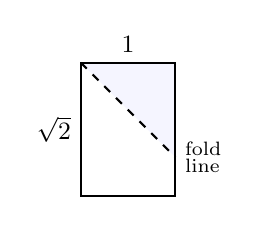
\begin{tikzpicture}[font=\small, baseline=(current bounding box.north)]
  \pgfmathsetmacro{\w}{1.2}
  \pgfmathsetmacro{\h}{1.2*sqrt(2)}
  \fill[blue!4] (0,\h) -- (\w,\h) -- (\w,\h-\w) -- cycle;
  \draw[thick] (0,0) rectangle (\w,\h);
  \draw[dashed, thick] (0,\h) -- (\w,\h-\w);
  \node[above] at (\w/2,\h) {$1$};
  \node[left] at (0,\h/2) {$\sqrt{2}$};
  \node[right, font=\scriptsize, align=left] at (\w,\h-\w)
    {fold\\[-2pt]line};
\end{tikzpicture}
\end{minipage}

\end{enumerate}

\newpage

\begin{ealglossed}
\parttitle{2}{New rules, new \ealgloss{ratios}{stosunki}}
\end{ealglossed}

\begin{ealglossed}
Each new rule for cutting a rectangle leads to a new \ealgloss{ratio}{stosunek}.
\end{ealglossed}

\begin{enumerate}[resume]

\item
\begin{ealglossed}
A card can be cut into three equal strips, each \ealgloss{similar}{podobny} to the whole card. The long side of the card is $x$. Find the \ealgloss{ratio}{stosunek} of the card, short : long.
\end{ealglossed}

\vspace{3pt}
\begin{minipage}[t]{0.30\linewidth}
\vspace{0pt}
\cutdiagram{3}{1.732}{$x$}{$?$}{cut}
\end{minipage}%
\begin{minipage}[t]{0.66\linewidth}
\vspace{2pt}
{\renewcommand{\arraystretch}{2}
\begin{tabular}{@{}l@{\qquad}l@{}}
Whole card, short : long & \ansline[1.4cm]\ $:$\ \ansline[1.4cm]\\
One strip, short : long  & \ansline[1.4cm]\ $:$\ \ansline[1.4cm]\\
\end{tabular}}
\end{minipage}

\vspace{2cm}
The card is $1:{}$\gap.

\item
\begin{enumerate}
  \item
  \begin{ealglossed}
  A card can be cut into five equal strips, each \ealgloss{similar}{podobny} to the whole card. Find its \ealgloss{ratio}{stosunek} short : long.
  \end{ealglossed}
  \item
  \begin{ealglossed}
  Write down the \ealgloss{ratio}{stosunek} for a card that cuts into $n$ \ealgloss{similar}{podobne} strips in the same way.
  \end{ealglossed}
  \item
  \begin{ealglossed}
  For which values of $n$ can the \ealgloss{ratio}{stosunek} be written with \ealgloss{whole numbers}{liczby całkowite nieujemne}? Draw an example, cut into its strips.
  \end{ealglossed}
\end{enumerate}

\item
\begin{minipage}[t]{0.74\linewidth}
\begin{ealglossed}
A rectangle is $1:x$. Cutting off the largest possible \ealgloss{square}{kwadrat} leaves a rectangle \ealgloss{similar}{podobny} to the whole rectangle. This is the \textbf{\ealgloss{golden rectangle}{złoty prostokąt}}.
\end{ealglossed}
\begin{enumerate}
  \item Fill in the gaps.

        \vspace{1pt}
        \begin{minipage}[t]{0.6\linewidth}
        \centering
        \worktitle{Left over, short : long}
        \bothsides{\eqgap \& : \& 1\\ 1 \& : \& \eqgap\\}{\div(x-1)}
        \end{minipage}
  \item Show that $x^2-x-1=0$.
  \item
  \begin{ealglossed}
  Use the fact $x^2-x-1=\left(x-\frac{1}{2}\right)^2-\frac{5}{4}$ to solve the \ealgloss{equation}{równanie} by \ealgloss{rearranging}{przekształcając}. Give the \ealgloss{ratio}{stosunek} of the \ealgloss{golden rectangle}{złoty prostokąt} exactly and to 3 \ealgloss{decimal places}{miejsca dziesiętne}.
  \end{ealglossed}
\end{enumerate}
\end{minipage}\hfill
\begin{minipage}[t]{0.22\linewidth}
\vspace{6pt}
\centering
\begin{ealglossed}
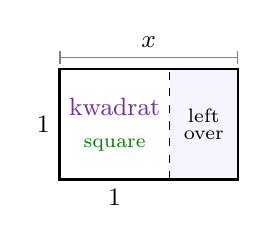
\begin{tikzpicture}[font=\small, baseline=(current bounding box.north)]
  \pgfmathsetmacro{\s}{1.4}
  \pgfmathsetmacro{\g}{1.4*1.618}
  \fill[blue!4] (\s,0) rectangle (\g,\s);
  \draw[thick] (0,0) rectangle (\g,\s);
  \draw[dashed] (\s,0) -- (\s,\s);
  \node[left] at (0,\s/2) {$1$};
  \node[below] at (\s/2,0) {$1$};
  \draw[|-|, gray] (0,\s+0.15) -- node[above, text=black] {$x$} (\g,\s+0.15);
  \node[font=\scriptsize] at (\s/2,\s/2) {\ealgloss{square}{kwadrat}};
  \node[font=\scriptsize, align=center] at ({(\s+\g)/2},\s/2)
    {left\\[-2pt]over};
\end{tikzpicture}
\end{ealglossed}
\end{minipage}

\item
\begin{minipage}[t]{0.74\linewidth}
\begin{ealglossed}
The largest possible \ealgloss{square}{kwadrat} is cut off a sheet of A4, $1:\sqrt{2}$.
\end{ealglossed}
\begin{enumerate}
  \item Write the rectangle left over as short : long.
  \item Fill in the gaps. (Hint: work out
        $\left(\sqrt{2}-1\right)\left(\sqrt{2}+1\right)$.)

        \vspace{1pt}
        \begin{minipage}[t]{0.6\linewidth}
        \centering
        \worktitle{Left over, short : long}
        \bothsides{\sqrt{2}-1 \& : \& 1\\ \eqgap \& : \& \eqgap\\}
          {\times\left(\sqrt{2}+1\right)}
        \end{minipage}
  \item
  \begin{ealglossed}
  A rectangle is $1:\left(1+\sqrt{2}\right)$. Show that cutting off two \ealgloss{squares}{kwadraty} leaves a rectangle \ealgloss{similar}{podobny} to the whole rectangle.
  \end{ealglossed}
\end{enumerate}
\end{minipage}\hfill
\begin{minipage}[t]{0.22\linewidth}
\vspace{6pt}
\centering
\begin{ealglossed}
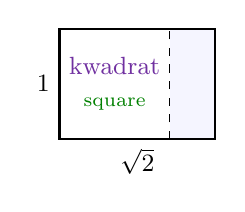
\begin{tikzpicture}[font=\small, baseline=(current bounding box.north)]
  \pgfmathsetmacro{\s}{1.4}
  \pgfmathsetmacro{\g}{1.4*sqrt(2)}
  \fill[blue!4] (\s,0) rectangle (\g,\s);
  \draw[thick] (0,0) rectangle (\g,\s);
  \draw[dashed] (\s,0) -- (\s,\s);
  \node[left] at (0,\s/2) {$1$};
  \node[below] at (\g/2,0) {$\sqrt{2}$};
  \node[font=\scriptsize] at (\s/2,\s/2) {\ealgloss{square}{kwadrat}};
\end{tikzpicture}
\end{ealglossed}
\end{minipage}

\end{enumerate}

\parttitle{3}{Other shapes}

\begin{enumerate}[resume]

\item
\begin{ealglossed}
Each shape is cut into equal pieces, and each piece is \ealgloss{similar}{podobny} to the whole shape. Find the \ealgloss{ratio}{stosunek} of lengths, piece : whole.
\end{ealglossed}

\vspace{2pt}
\begin{minipage}[b]{0.31\linewidth}
\centering
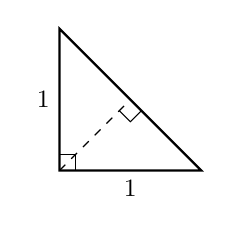
\begin{tikzpicture}[font=\small]
  \pgfmathsetmacro{\a}{1.8}
  \draw[thick] (0,0) -- (\a,0) -- (0,\a) -- cycle;
  \draw[dashed] (0,0) -- (\a/2,\a/2);
  \draw (0.2,0) -- (0.2,0.2) -- (0,0.2);
  \draw ({\a/2-0.14},{\a/2-0.14}) -- ({\a/2},{\a/2-0.28})
    -- ({\a/2+0.14},{\a/2-0.14});
  \node[below] at (\a/2,0) {$1$};
  \node[left] at (0,\a/2) {$1$};
\end{tikzpicture}

\small (a) Two pieces
\end{minipage}\hfill
\begin{minipage}[b]{0.36\linewidth}
\centering
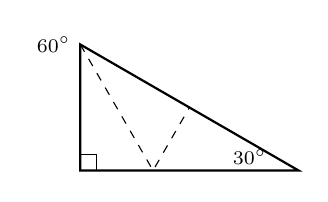
\begin{tikzpicture}[font=\small]
  \pgfmathsetmacro{\s}{1.6}
  \coordinate (C) at (0,0);
  \coordinate (A) at ({\s*sqrt(3)},0);
  \coordinate (B) at (0,\s);
  \coordinate (D) at ({\s/sqrt(3)},0);
  \coordinate (E) at ({\s*sqrt(3)/2},{\s/2});
  \draw[thick] (C) -- (A) -- (B) -- cycle;
  \draw[dashed] (B) -- (D) -- (E);
  \draw (0.2,0) -- (0.2,0.2) -- (0,0.2);
  \node[font=\scriptsize] at ({\s*sqrt(3)-0.62},0.17) {$30^\circ$};
  \node[font=\scriptsize, left] at (B) {$60^\circ$};
\end{tikzpicture}

\small (b) Three pieces
\end{minipage}\hfill
\begin{minipage}[b]{0.31\linewidth}
\centering
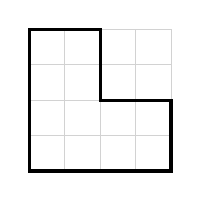
\begin{tikzpicture}[scale=0.45]
  \draw[gray!35] (0,0) grid (4,4);
  \draw[very thick] (0,0) -- (4,0) -- (4,2) -- (2,2) -- (2,4) -- (0,4) -- cycle;
\end{tikzpicture}

\small (c) Four pieces: draw them
\end{minipage}

\begin{enumerate}
  \setcounter{enumii}{3}
  \item
  \begin{ealglossed}
  A shape is cut into $n$ equal pieces like this. Explain why the \ealgloss{ratio}{stosunek} of lengths, piece : whole, is $1:\sqrt{n}$. Use this to explain why A4 is $1:\sqrt{2}$ in a different way.

  Fill in the hint first: if every length is multiplied by $k$, then the \ealgloss{area}{pole} is \ansline[3.5cm].
  \end{ealglossed}
\end{enumerate}

\end{enumerate}

\newpage

\begin{ealglossed}
\parttitle{4}{More \ealgloss{dimensions}{wymiary}, and patterns}
\end{ealglossed}

\begin{enumerate}[resume]

\item
\begin{ealglossed}
A block of cheese is a \ealgloss{cuboid}{prostopadłościan} with \ealgloss{edges}{krawędzie} $1:y:z$, from shortest to longest. Halving its longest \ealgloss{edge}{krawędź} cuts it into two blocks \ealgloss{similar}{podobne} to the whole block.
\end{ealglossed}

\begin{minipage}[t]{0.66\linewidth}
\begin{enumerate}
  \item Fill in the gaps.

        \vspace{1pt}
        \begin{center}
        \worktitle{Half block, shortest : middle : longest}
        \bothsides[ratio3]{\eqgap \& : \& 1 \& : \& y\\
          \eqgap \& : \& \eqgap \& : \& \eqgap\\
          1 \& : \& \eqgap \& : \& \eqgap\\}{\times2, \div z}
        \end{center}
  \item
  \begin{ealglossed}
  The blocks are \ealgloss{similar}{podobne}, so $1:y:z$ is equal to your last line. Use this to show that $y^3=2$.
  \end{ealglossed}
\end{enumerate}
\end{minipage}\hfill
\begin{minipage}[t]{0.30\linewidth}
\vspace{4pt}
\centering
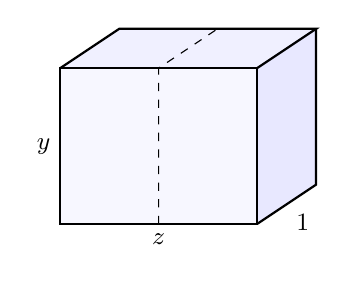
\begin{tikzpicture}[font=\small, baseline=(current bounding box.north)]
  \pgfmathsetmacro{\Z}{2.5}
  \pgfmathsetmacro{\Y}{1.98}
  \pgfmathsetmacro{\dx}{0.75}
  \pgfmathsetmacro{\dy}{0.5}
  \fill[blue!3] (0,0) rectangle (\Z,\Y);
  \fill[blue!6] (0,\Y) -- (\dx,\Y+\dy) -- (\Z+\dx,\Y+\dy) -- (\Z,\Y) -- cycle;
  \fill[blue!9] (\Z,0) -- (\Z+\dx,\dy) -- (\Z+\dx,\Y+\dy) -- (\Z,\Y) -- cycle;
  \draw[thick] (0,0) rectangle (\Z,\Y);
  \draw[thick] (0,\Y) -- (\dx,\Y+\dy) -- (\Z+\dx,\Y+\dy) -- (\Z,\Y);
  \draw[thick] (\Z,0) -- (\Z+\dx,\dy) -- (\Z+\dx,\Y+\dy);
  \draw[dashed] (\Z/2,0) -- (\Z/2,\Y) -- (\Z/2+\dx,\Y+\dy);
  \node[below] at (\Z/2,0) {$z$};
  \node[left] at (0,\Y/2) {$y$};
  \node[below right] at (\Z+\dx/2,\dy/2) {$1$};
\end{tikzpicture}
\end{minipage}

\begin{enumerate}
  \setcounter{enumii}{2}
  \item
  \begin{ealglossed}
  Find the \ealgloss{ratio}{stosunek} $1:y:z$ exactly and to 3 \ealgloss{decimal places}{miejsca dziesiętne}.
  \end{ealglossed}
  \item
  \begin{ealglossed}
  A block has a \ealgloss{volume}{objętość} of $1$ litre ($1000\text{ cm}^3$). Find its \ealgloss{edges}{krawędzie}, and show that one is $10$\,cm.
  \end{ealglossed}
\end{enumerate}

\item
\begin{ealglossed}
We cannot draw a \textbf{\ealgloss{four-dimensional}{czterowymiarowy} box}, but we can describe one: it has four \ealgloss{edges}{krawędzie}, each at \ealgloss{right angles}{kąty proste} to all the others. One has \ealgloss{edges}{krawędzie} $1:a:b:c$, from shortest to longest. Halving its longest \ealgloss{edge}{krawędź} gives two boxes \ealgloss{similar}{podobne} to the whole box.
\end{ealglossed}
\begin{enumerate}
  \item Write the half box, shortest : \ldots : longest, in the form
        $1:\ldots:\ldots:\ldots$
  \item Show that $b=a^2$ and $c=a^3$, and that $a^4=2$.
  \item
  \begin{ealglossed}
  Find the \ealgloss{ratio}{stosunek} $1:a:b:c$ to 3 \ealgloss{decimal places}{miejsca dziesiętne}. One of these numbers appears earlier on this sheet. Where, and why?
  \end{ealglossed}
\end{enumerate}

\item
\begin{ealglossed}
A rectangle, box or \ealgloss{four-dimensional}{czterowymiarowy} box is cut into equal slices across its longest \ealgloss{edge}{krawędź}, and each slice is \ealgloss{similar}{podobny} to the whole shape. Its \ealgloss{edges}{krawędzie} are then in the \ealgloss{ratio}{stosunek} $1:r:r^2:\ldots$
\end{ealglossed}
\begin{enumerate}
  \item Complete the table of the values of $r$. Some of them have been found
        already on this sheet.

        \vspace{1pt}
        {\small\renewcommand{\arraystretch}{1.3}
        \begin{tabular}{|l|*{4}{C{2.75cm}|}}
        \hline
        & \textbf{Rectangle (2D)} & \textbf{Box (3D)} & \textbf{4D box}
          & \textbf{$d$ \ealgloss{dimensions}{wymiary}}\\ \hline
        \textbf{2 slices} & $\sqrt{2}$ & & & \\ \hline
        \textbf{3 slices} & & & & \\ \hline
        \textbf{$n$ slices} & & & & \\ \hline
        \end{tabular}}
  \item
  \begin{ealglossed}
  For 2 slices, work out longest \ealgloss{edge}{krawędź} $\div$ shortest \ealgloss{edge}{krawędź} in 2, 3, 4 and 10 \ealgloss{dimensions}{wymiary}.
  \end{ealglossed}
  \item
  \begin{ealglossed}
  What happens to longest \ealgloss{edge}{krawędź} $\div$ shortest \ealgloss{edge}{krawędź} as the number of \ealgloss{dimensions}{wymiary} gets larger? Explain why it is always less than $2$. (Hint: $r^{d-1}=r^d\div r$.)
  \end{ealglossed}
\end{enumerate}

\item
\begin{ealglossed}
A rectangle is $1:x$. Cutting off $k$ \ealgloss{squares}{kwadraty} leaves a \ealgloss{similar}{podobny} rectangle. (Q11 is $k=1$ and Q12 is $k=2$.)
\end{ealglossed}
\begin{enumerate}
  \item Show that $x^2-kx-1=0$.
  \item
  \begin{ealglossed}
  Use the fact
        $x^2-kx-1=\left(x-\frac{k}{2}\right)^2-\frac{k^2+4}{4}$ to solve
        $x^2-3x-1=0$ by \ealgloss{rearranging}{przekształcając}. Give the \ealgloss{ratio}{stosunek} when $k=3$, exactly and to 3 \ealgloss{decimal places}{miejsca dziesiętne}.
  \end{ealglossed}
  \item
  \begin{ealglossed}
  \ealgloss{Rearrange}{Przekształć} $\left(x-\frac{k}{2}\right)^2-\frac{k^2+4}{4}=0$ to find $x$ \ealgloss{in terms of}{w zależności od} $k$. Check it with Q11 and Q12.
  \end{ealglossed}
  \item
  \begin{ealglossed}
  Invent your own rule for cutting a rectangle, a triangle or a box into pieces, so that one or more of the pieces is \ealgloss{similar}{podobny} to the whole shape. Find the \ealgloss{ratio}{stosunek} that your rule leads to.
  \end{ealglossed}
\end{enumerate}

\item
\begin{minipage}[t]{0.64\linewidth}
The diagram shows a sheet of A0 cut into one sheet of each size from A1 to
A6, with one more sheet of A6 left over.
\begin{enumerate}
  \item
  \begin{ealglossed}
  What is the total \ealgloss{area}{pole} of the sheets from A1 to A6, in m$^2$?
  \end{ealglossed}
  \item
  \begin{ealglossed}
  The pattern carries on forever, to A7, A8, A9 and so on. What happens to the total \ealgloss{area}{pole} of all the sheets? Explain why.
  \end{ealglossed}
  \item For lengths, A0 : A10 $=1:\left(\frac{1}{\sqrt{2}}\right)^{10}$. Show
        that this is $1:\frac{1}{32}$, and find the size of A10.
\end{enumerate}
\end{minipage}\hfill
\begin{minipage}[t]{0.33\linewidth}
\vspace{2pt}
\centering
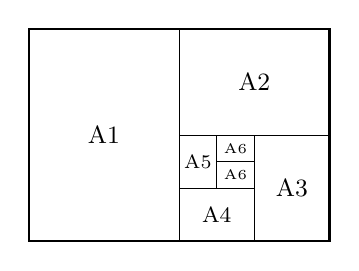
\begin{tikzpicture}[font=\small, baseline=(current bounding box.north)]
  \pgfmathsetmacro{\H}{2.7}
  \pgfmathsetmacro{\W}{2.7*sqrt(2)}
  \draw[thick] (0,0) rectangle (\W,\H);
  \draw (\W/2,0) -- (\W/2,\H);
  \draw (\W/2,\H/2) -- (\W,\H/2);
  \draw (3*\W/4,0) -- (3*\W/4,\H/2);
  \draw (\W/2,\H/4) -- (3*\W/4,\H/4);
  \draw (5*\W/8,\H/4) -- (5*\W/8,\H/2);
  \draw (5*\W/8,3*\H/8) -- (3*\W/4,3*\H/8);
  \node at (\W/4,\H/2) {A1};
  \node at (3*\W/4,3*\H/4) {A2};
  \node at (7*\W/8,\H/4) {A3};
  \node[font=\footnotesize] at (5*\W/8,\H/8) {A4};
  \node[font=\scriptsize] at (9*\W/16,3*\H/8) {A5};
  \node[font=\tiny] at (11*\W/16,7*\H/16) {A6};
  \node[font=\tiny] at (11*\W/16,5*\H/16) {A6};
\end{tikzpicture}
\end{minipage}

\end{enumerate}

\end{document}